% !TEX program = xelatex
\documentclass[a4paper,12pt]{article}

\usepackage{fontspec}
\usepackage{microtype}
\usepackage{graphicx}
\usepackage{booktabs}
\usepackage{longtable}
\usepackage{xcolor}
\usepackage{fancyvrb}
\usepackage[a4paper,margin=2.2cm]{geometry}
\usepackage[unicode=true,colorlinks=true,linkcolor=black,citecolor=black,
            urlcolor=black,bookmarksnumbered=true]{hyperref}
\usepackage{bookmark}
\usepackage{xurl}

\usepackage{xepersian}

\IfFontExistsTF{Vazirmatn}{\settextfont[Ligatures=TeX]{Vazirmatn}}{%
  \IfFontExistsTF{Shabnam}{\settextfont[Ligatures=TeX]{Shabnam}}{%
    \IfFontExistsTF{Sahel}{\settextfont[Ligatures=TeX]{Sahel}}{%
      \IfFontExistsTF{Amiri}{\settextfont[Ligatures=TeX]{Amiri}}{%
        \settextfont[Ligatures=TeX]{DejaVu Sans}}}}}
\IfFontExistsTF{TeX Gyre Termes}{%
  \setlatintextfont{TeX Gyre Termes}}{%
  \IfFontExistsTF{Liberation Serif}{%
    \setlatintextfont{Liberation Serif}}{%
    \setlatintextfont{DejaVu Serif}}}
\IfFontExistsTF{Vazirmatn}{\setdigitfont{Vazirmatn}}{%
  \IfFontExistsTF{Shabnam}{\setdigitfont{Shabnam}}{%
    \IfFontExistsTF{Sahel}{\setdigitfont{Sahel}}{%
      \IfFontExistsTF{Amiri}{\setdigitfont{Amiri}}{%
        \setdigitfont{DejaVu Sans}}}}}
\IfFontExistsTF{TeX Gyre Cursor}{\setmonofont[Scale=0.92]{TeX Gyre Cursor}}{%
  \IfFontExistsTF{DejaVu Sans Mono}{\setmonofont[Scale=0.90]{DejaVu Sans Mono}}{%
    \setmonofont[Scale=0.90]{Liberation Mono}}}

\newcommand{\en}[1]{\lr{#1}}
\pdfstringdefDisableCommands{\def\lr#1{#1}\def\en#1{#1}}

\emergencystretch=2em
\setlength{\parskip}{0.4em}

\begin{document}

\title{\en{NGINX} در یک \en{cloud infrastructure}}
\author{}
\date{}
\maketitle

\section*{فهرست مطالب این فصل}

\begin{itemize}
\item درک \en{cloud infrastructure}
\item استفاده از \en{Docker}
\item راه‌اندازی \en{NGINX} داخل \en{Docker}
\item راه‌اندازی \en{NGINX} داخل \en{Docker} برای \en{proxy} کردن
      \en{application}های روی \en{host}
\end{itemize}

در زیرساخت وب، حرکت از \en{server configuration} سنتی به معماری ابری دیگر
بحث نظری نیست. در \en{deployment}های قدیمی، \en{server} را دستی
\en{configure} می‌کردند تا چند سایت یا برنامه را نگه دارد. حالا روش‌های
ابرمحورِ چابک‌تر و مقیاس‌پذیرتر جایش را گرفته‌اند. این فصل روی کار عملی
پذیرش \en{cloud infrastructure} تمرکز می‌کند: مدیریت بهتر منابع، امنیت
قوی‌تر، و کنترل ساده‌تر ترافیک بالا.

اینجا نقش \en{NGINX} را در همان فضا می‌بینیم و \en{Docker} را بستر کار
می‌گیریم. با کنار هم گذاشتن \en{NGINX} و \en{Docker} نشان می‌دهیم چند
\en{service} را چطور هماهنگ راه بیندازید تا محیط پایدارتر و انعطاف‌پذیرتری
بسازید. اگر \en{Docker} برایتان تازه است هم اشکالی ندارد؛ قدم‌به‌قدم اولین
تجربه را با محوریت \en{NGINX} پیش می‌بریم تا ورود به
\en{containerized deployment} روشن بماند.

\section{درک \en{cloud infrastructure}}

امروز \en{cloud service}ها بخشی از کار روزمرهٔ آنلاین شده‌اند. اپ موبایل با نسخهٔ
رومیزی هم‌گام می‌شود و همان \en{server} آشنا تبدیل شده به ابری که برای کاربر
ساده‌تر است، ولی زیرساخت وب را پیچیده‌تر می‌کند. این تغییر، ذخیره و کار با
داده را عوض کرده و ما را به وضعیتی همیشه متصل و ابرمحور برده است.

\subsection{رویکرد سنتی}

برای فهم جزئیات \en{cloud infrastructure}، اول سراغ چیدمان سنتی برویم و با
نگاه امروزی به آن نگاه کنیم. \en{WordPress} را در نظر بگیرید: سکوی متن‌باز
ساخت وب‌سایت که روی یک \en{web server}، یک \en{PHP server} و یک
\en{database server} اجرا می‌شود. روش کلاسیک این است که هر سه را روی یک
ماشین نصب کنید؛ برای میزبانی یک وبلاگ تنها، راه‌حل ساده‌ای است:

\begin{figure}[ht]
\centering
\begin{LTR}
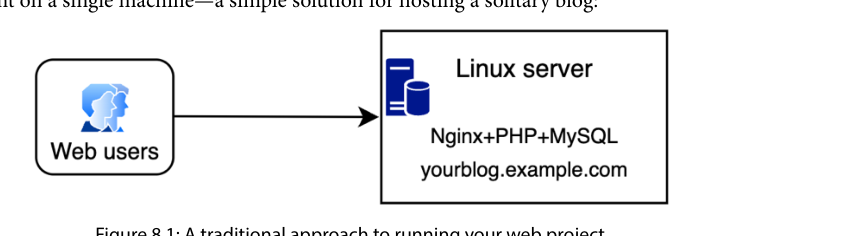
\includegraphics[width=0.92\linewidth]{figures/fig-8-1.png}
\end{LTR}
\caption{شکل \lr{8.1}: رویکرد سنتی برای اجرای پروژهٔ وب}
\end{figure}

ولی وقتی مقیاس بزرگ‌تر می‌شود، محدودیت‌ها دیده می‌شود. وابستگی‌های نرم‌افزاری
گاهی چند نسخهٔ متناقض می‌خواهند و کنار هم ماندنشان سخت است. هرچه
\en{service}ها بیشتر شوند، مدیریت همه روی یک \en{server} هم دشوارتر می‌شود.

\subsection{رویکرد ابری}

وقتی چند \en{service} را روی یک \en{server} می‌خواهید، مشکل تکراری
وابستگی‌های ناسازگار پیش می‌آید. فرض کنید یکی به \en{PHP 7.4} نیاز دارد و
دیگری به \en{PHP 8.3}. ابزار \en{Docker} این را با بسته‌بندی برنامه‌ها در
\en{container} حل می‌کند: محیط‌های جدا که به نسخهٔ نرم‌افزارهای
\en{Linux distribution} زیرین وابسته نیستند.

مزیت‌های \en{container}های \en{Docker} از این قرارند:

\begin{itemize}
\item \textbf{مدیریت نسخه:} نگهداشت و عوض کردن نسخه ساده‌تر می‌شود و برگشت
      به عقب هم راحت‌تر است.
\item \textbf{ایزوله‌سازی و کارایی:} برنامه‌ها از هم جدا می‌مانند؛ هم
      جابه‌جایی آسان‌تر می‌شود، هم مصرف منابع یکی روی بقیه اثر نمی‌گذارد.
\item \textbf{ساده‌تر شدن \en{deployment}:} بعد از عبور از منحنی یادگیری
      \en{Docker}، \en{deployment} و مقیاس‌پذیری مدیریت‌پذیرتر می‌شود و
      انعطافی می‌دهد که در چیدمان سنتی کمتر دیده می‌شود.
\end{itemize}

همان سناریوی وبلاگ را دوباره ببینیم، این‌بار با \en{Docker}:

\begin{figure}[ht]
\centering
\begin{LTR}
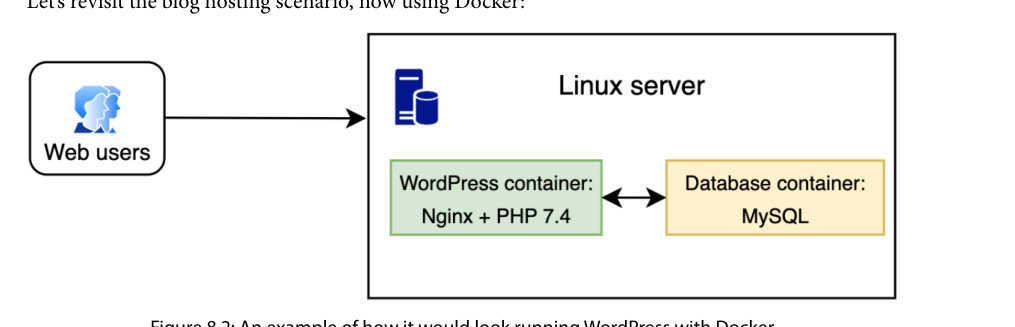
\includegraphics[width=0.92\linewidth]{figures/fig-8-2.png}
\end{LTR}
\caption{شکل \lr{8.2}: نمونه‌ای از اجرای \en{WordPress} با \en{Docker}}
\end{figure}

\en{server} یک \en{Linux distribution} دارد و روی آن دو \en{container}
جدا مثل محیط‌های مینیمال \en{Linux} عمل می‌کنند؛ هر کدام فقط همان چیزی را
دارد که برای اجرای برنامه‌اش لازم است.

اگر \en{service}ای مثل \en{Nextcloud} با \en{PHP 8.3} را کنار
\en{WordPress} روی \en{PHP 7.4} اضافه کنید، همان توانایی \en{Docker} را
می‌بینید:

\begin{figure}[ht]
\centering
\begin{LTR}
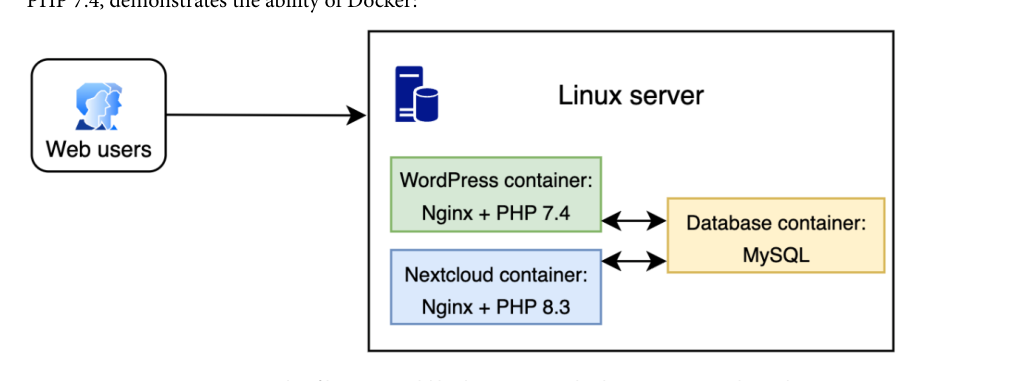
\includegraphics[width=0.92\linewidth]{figures/fig-8-3.png}
\end{LTR}
\caption{شکل \lr{8.3}: نمونه‌ای از اجرای چند \en{container} با \en{Docker}}
\end{figure}

چنان‌که در شکل دیده می‌شود، این چیدمان اجازه می‌دهد خیلی از
\en{Docker image}ها، هر کدام با نسخهٔ نرم‌افزار خودش، هم‌زمان در محیط ایزوله
اجرا شوند. اگر در یک \en{container} مشکل امنیتی پیش بیاید، اثرش همان‌جا
می‌ماند و بقیهٔ سیستم محفوظ‌تر است.

موضوع‌های پیشرفته مثل \en{Docker Swarm} برای
\en{high availability (HA)} یا \en{Kubernetes} برای مقیاس‌پذیری در این فصل
نیست؛ ولی برای جلو بردن \en{cloud infrastructure} ارزش پیگیری دارند.

\section{استفاده از \en{Docker}}

در بخش قبل پایه‌های معماری ابری را دیدیم. حالا از نظریه به عمل می‌رویم:
\en{Docker} را قدم‌به‌قدم نصب و \en{configure} می‌کنیم تا اولین
\en{container} را بالا بیاوریم.

\en{Docker} فقط یک ابزار نیست؛ تغییر الگوی کار است: نرم‌افزار بسته‌بندی و
ایزوله می‌شود تا در محیط‌های مختلف یکسان بماند. تا پایان این بخش،
\en{Docker} دیگر مفهوم صرف نیست؛ بخشی از جعبه‌ابزار شماست و کار را با
\en{deployment} یک \en{container} برای \en{NGINX} شروع می‌کنیم.

\subsection{نصب \en{Docker}}

خوشبختانه تیم \en{Docker} اسکریپتی گذاشته که نصب را ساده می‌کند. این
اسکریپت با توزیع‌های رایج \en{Linux} سازگار است؛ از جمله
\en{Red Hat Enterprise Linux (RHEL)}، \en{CentOS}، \en{Fedora}،
\en{Debian}، \en{Ubuntu} و مشتق‌هایشان.

برای نصب، اسکریپت را با دسترسی \en{root} اجرا کنید. در ترمینال این \en{command} را
بزنید:

\begin{latin}
\begin{Verbatim}[fontsize=\small,frame=single,framesep=6pt,baselinestretch=1.1]
# curl -s https://get.docker.com | bash
\end{Verbatim}
\end{latin}

با همین یک \en{command}، \en{Docker} با مخزن‌های سفارشی متناسب با
\en{package manager} توزیع شما نصب می‌شود. یعنی به‌روزرسانی \en{Docker}
مثل به‌روزرسانی بقیهٔ بسته‌های سیستم ساده می‌ماند.

\subsection{اولین \en{container} با \en{Docker}}

برای کار با \en{container} راه‌های زیادی هست. مثلاً می‌توانید با یک \en{command}
ساده یک \en{container} راه بیندازید:

\begin{latin}
\begin{Verbatim}[fontsize=\small,frame=single,framesep=6pt,baselinestretch=1.1]
root@docker:~# docker run -d nginx
latest: Pulling from library/nginx
e1caac4eb9d2: Pull complete
\end{Verbatim}
\end{latin}

این \en{command}، \en{image} مربوط به \en{NGINX} را از \en{Docker Hub} می‌کشد و
\en{container} تازه‌ای را در \en{detached mode} شروع می‌کند. ولی این
\en{container} با تنظیم پیش‌فرض بالا می‌آید و هنوز برای کار مشخصی
\en{configure} نشده است.

برای سفارشی‌سازی می‌توانید پارامترهای بیشتری بدهید. مثلاً برای نگاشت
\en{port} شمارهٔ \lr{80} داخل \en{container} به \en{port} شمارهٔ \lr{80}
روی \en{host} تا ترافیک وب برسد:

\begin{latin}
\begin{Verbatim}[fontsize=\small,frame=single,framesep=6pt,baselinestretch=1.1]
root@docker:~# docker run -d nginx -p 80:80
\end{Verbatim}
\end{latin}

\en{command} اول \en{container} مربوط به \en{NGINX} را با \en{configuration} پیش‌فرض راه
می‌اندازد. \en{command} دوم همان را اجرا می‌کند، ولی این‌بار از \en{port}
شمارهٔ \lr{80} ماشین \en{host} در دسترس است. اگر \en{configuration} کامل‌تری لازم
دارید، نوبت \en{Docker Compose} است: مدیریت چند \en{container} در یک
برنامهٔ \en{Docker} را ساده‌تر می‌کند.

در فضای این کتاب، \en{image} مربوط به \en{NGINX} نمونهٔ خوبی از توان
\en{Docker} است؛ چون نشان می‌دهد \en{containerization} چطور
\en{deployment} را برای \en{service}هایی که معمولاً \en{server}
اختصاصی می‌خواهند ساده می‌کند.

در ادامه می‌بینیم چطور یک \en{container} برای \en{NGINX} را تنظیم کنید تا
محتوای ایستا بدهد یا به‌عنوان \en{reverse proxy} کار کند. آنجا سراغ مفهوم
\en{Docker volume} می‌رویم و می‌بینیم چطور فایل \en{configuration} و محتوا را با آن
سرو کنید.

\subsection{ساده‌سازی با \en{Docker Compose}}

بعد از اولین \en{container} روشن شد که مدیریت پارامترها مستقیم از خط \en{command}
زود شلوغ می‌شود. \en{Docker Compose} این کار را ساده می‌کند: تعریف و اجرای
برنامه‌های چند\en{container}ای \en{Docker} با یک فایل \en{YAML}.

معادل همان چیدمان قبلی را بسازیم: یک \en{container} برای \en{NGINX} با
\en{port} شمارهٔ \lr{80} در دسترس \en{host}.

\begin{enumerate}
\item اول پوشهٔ \en{/root/nginx} را بسازید و داخلش فایلی به نام
\en{docker-compose.yml} با این محتوا ذخیره کنید:

\begin{latin}
\begin{Verbatim}[fontsize=\small,frame=single,framesep=6pt,baselinestretch=1.1]
version: '3'
services:
  nginx:
    image: nginx:latest
    ports:
      - "80:80"
\end{Verbatim}
\end{latin}

\begin{quote}
\textbf{یادآوری}\\
قالب فایل \en{YAML} نام دارد، ولی پسوند باید \en{.yml} باشد.
\end{quote}

% fa-lint: allow terminology-drift
در این \en{docker-compose.yml} یک \en{service} به نام \en{nginx} تعریف
% fa-lint: allow terminology-drift
کرده‌ایم که از \en{image} رسمی \en{nginx} با برچسب \en{latest} استفاده
می‌کند؛ یعنی هر بار از \en{Docker Hub} بکشید به‌روز می‌شود. اگر بخواهید
می‌توانید نسخهٔ ثابت بگذارید، مثلاً \en{nginx:1.25.4}. جزئیات بیشتر در
صفحهٔ \en{Docker Hub} برای \en{NGINX} هست
(\en{https://hub.docker.com/\_/nginx/}).

\item حالا با فایل ذخیره‌شده، در همان پوشه این \en{command} را بزنید:

\begin{latin}
\begin{Verbatim}[fontsize=\small,frame=single,framesep=6pt,baselinestretch=1.1]
root@nginx:~/nginx# docker compose up
[+] Running 1/1
 ✔ Container nginx-nginx-1  Created
\end{Verbatim}
\end{latin}

\item همین الان اولین \en{container} را با \en{Docker Compose} بالا
آوردید. برای توقف، \en{Ctrl+C (\^{}C)} کافی است. یا در \en{detached mode} با
\en{up -d} شروع کنید و با \en{down} متوقف کنید:

\begin{latin}
\begin{Verbatim}[fontsize=\small,frame=single,framesep=6pt,baselinestretch=1.1]
root@nginx:~/nginx# docker compose up -d
root@nginx:~/nginx# docker compose down
\end{Verbatim}
\end{latin}
\end{enumerate}

با \en{Docker Compose}، اجرای \en{NGINX} در \en{Docker} می‌شود تعریف وضعیت
مطلوب در یک فایل؛ خواندن و نگهداشتش از \en{command}های پراکنده آسان‌تر است. در بخش
بعد \en{NGINX} داخل \en{Docker} را بیشتر برای نیاز خودمان تنظیم می‌کنیم.

\section{راه‌اندازی \en{NGINX} داخل \en{Docker}}

حالا که با \en{Docker Compose} راحت‌ترید، \en{container} را جلوتر می‌بریم.
در این بخش \en{configuration} و محتوای سایت را به \en{container} مربوط به \en{NGINX}
اضافه می‌کنیم.

اول همان \en{docker-compose.yml} قبلی را دوباره ببینید. آنجا \en{service}
مربوط به \en{NGINX} آمده و \en{port} شمارهٔ \lr{80} داخل \en{container} به
\en{port} شمارهٔ \lr{80} روی \en{host} نگاشت شده تا وب‌سرور از \en{host}
دیده شود.

قدم بعد این است که \en{container} سایت را با فایل \en{configuration} و محتوای واقعی
روی ماشین \en{host} سرو کند. برای این کار از \en{Docker volume} استفاده
می‌کنیم. \en{volume} سازوکار ترجیحی برای ماندگاری داده‌ای است که
\en{container} می‌سازد و مصرف می‌کند. نمونهٔ تغییر
\en{docker-compose.yml} برای اتصال \en{volume}:

\begin{latin}
\begin{Verbatim}[fontsize=\small,frame=single,framesep=6pt,baselinestretch=1.1]
version: '3'
services:
  nginx:
    image: nginx:latest
    ports:
      - "80:80"
    volumes:
      - ./config/nginx.conf:/etc/nginx/nginx.conf
      - ./html:/usr/share/nginx/html
\end{Verbatim}
\end{latin}

اینجا \en{./config/nginx.conf} مسیر فایل \en{configuration} سفارشی \en{NGINX} روی
\en{host} است و \en{/etc/nginx/nginx.conf} جایی است که \en{container}
انتظار دارد \en{configuration} را ببیند. \en{volume} دوم، \en{./html}، پوشهٔ محتوای
سایت روی \en{host} است که داخل \en{container} روی
\en{/usr/share/nginx/html/} سوار می‌شود.

با این روش \en{configuration} یا محتوا را مستقیم روی \en{host} ویرایش می‌کنید و همان
تغییر داخل \en{container} دیده می‌شود.

\begin{quote}
\textbf{نکته}\\
\en{NGINX} از قبل \en{configuration} دارد؛ پس می‌توانید اتصال \en{volume} مربوط به
\en{nginx.conf} را نگذارید و از تنظیم پیش‌فرض استفاده کنید. پوشهٔ \en{html}
را حتماً وصل کنید؛ همان‌جاست که \en{NGINX} محتوای وب را برای سرو کردن
می‌جوید.
\end{quote}

\section{ادغام \en{PHP} با \en{NGINX} به‌کمک \en{Docker Compose}}

قدم بعد این است که \en{NGINX} محتوای پویا با \en{PHP} را هم هندل کند. این
ترکیب در توسعهٔ وب رایج است و \en{implementation} را با \en{Docker Compose} را ساده
می‌کند.

اول \en{docker-compose.yml} موجود را با یک \en{service} برای \en{PHP}
گسترش می‌دهیم؛ بعد مطمئن می‌شویم \en{NGINX} از راه \en{FastCGI} با آن حرف
می‌زند.

\begin{enumerate}
\item اول یک \en{service} برای \en{PHP} اضافه کنید که
\en{FastCGI Process Manager (php-fpm)} را اجرا کند. نمونهٔ
\en{docker-compose.yml} به‌روز شده:

\begin{latin}
\begin{Verbatim}[fontsize=\small,frame=single,framesep=6pt,baselinestretch=1.1]
version: '3'
services:
  nginx:
    image: nginx:latest
    ports:
      - "80:80"
    volumes:
      - ./config/nginx.conf:/etc/nginx/nginx.conf
      - ./html:/usr/share/nginx/html
    depends_on:
      - php
  php:
    image: php:8.3-fpm
    volumes:
      - ./html:/usr/share/nginx/html
\end{Verbatim}
\end{latin}

% fa-lint: allow terminology-drift
اینجا \en{service} با نام \en{php} از \en{image} رسمی \en{PHP} با
\en{php-fpm} استفاده می‌کند. پوشهٔ \en{html} را هم داخل همین
\en{container} سوار می‌کنیم تا به همان فایل‌های وبِ \en{NGINX} دسترسی
داشته باشد.

\item پیش از روشن کردن \en{container}ها باید ارتباط \en{NGINX} و \en{PHP}
را درست کنید. \en{nginx.conf} را ویرایش کنید و پارامترهای \en{FastCGI} را
بگذارید. نمونه:

\begin{latin}
\begin{Verbatim}[fontsize=\small,frame=single,framesep=6pt,baselinestretch=1.1]
events {}
http {
  server {
    listen 80;
    server_name localhost;

    root /usr/share/nginx/html;
    index index.php index.html index.htm;

    location / {
      try_files $uri $uri/ =404;
    }

    location ~ \.php$ {
      try_files $uri =404;
      fastcgi_pass php:9000;
      fastcgi_index index.php;
      fastcgi_param SCRIPT_FILENAME $document_root$fastcgi_script_name;
      include fastcgi_params;
    }
  }
}
\end{Verbatim}
\end{latin}

این \en{configuration} به \en{NGINX} می‌گوید درخواست فایل‌های \en{PHP} را به
% fa-lint: allow terminology-drift
\en{service} مربوط به \en{php-fpm} داخل \en{container} به نام \en{php}
بفرستد.

\begin{quote}
\textbf{توجه}\\
% fa-lint: allow terminology-drift
\en{NGINX} نام \en{service} مربوط به \en{php} را با \en{DNS} داخلی
\en{Docker} پیدا می‌کند تا با \en{php-fpm} حرف بزند. اگر نام \en{service}
را در \en{docker-compose.yml} عوض کردید، \en{nginx.conf} را هم همان‌طور
به‌روز کنید.
\end{quote}

\item با این \en{docker-compose.yml} و \en{nginx.conf} می‌توانید
\en{docker compose up} را بزنید؛ \en{NGINX} هم محتوای ایستا و هم صفحه‌های
پویای \en{PHP} را سرو می‌کند:

\begin{latin}
\begin{Verbatim}[fontsize=\small,frame=single,framesep=6pt,baselinestretch=1.1]
root@nginx:~/nginx# docker compose up
[+] Running 2/0
 ✔ Container docker-php-1    Created
 ✔ Container docker-nginx-1  Created
Attaching to nginx-1, php-1
php-1 [02-Mar-2024 11:42:30] NOTICE: fpm is running, pid 1
\end{Verbatim}
\end{latin}

\item بعد از بالا آمدن \en{container}ها، برای اطمینان از ارتباط درست
\en{NGINX} و \en{PHP}، فایلی بسازید با
\en{<?php phpinfo(); ?>}. با باز کردن آن صفحهٔ اطلاعات \en{PHP} دیده
می‌شود و ارتباط بین \en{container}ها تأیید می‌شود:

\begin{figure}[ht]
\centering
\begin{LTR}
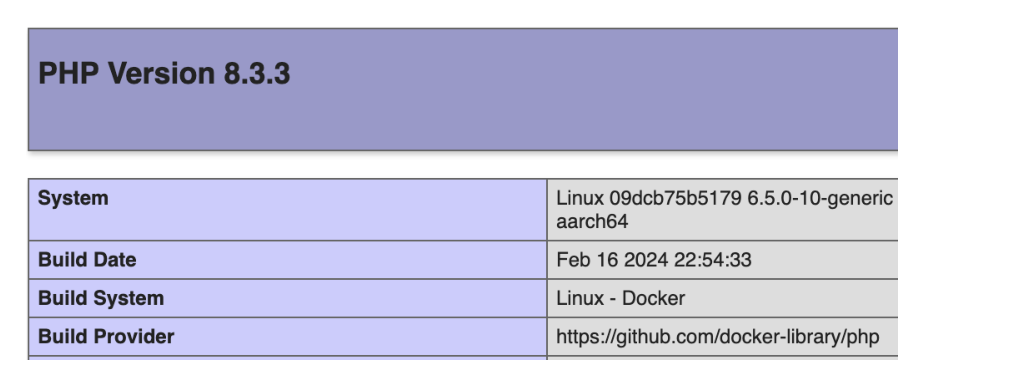
\includegraphics[width=0.92\linewidth]{figures/fig-8-4.png}
\end{LTR}
\caption{شکل \lr{8.4}: اجرای \en{phpinfo} داخل \en{Docker}}
\end{figure}
\end{enumerate}

این زیربخش افزودن \en{service} مربوط به \en{PHP} به محیط \en{Docker} و
\en{configuration} مربوط به \en{NGINX} برای پردازش اسکریپت‌های \en{PHP} از راه \en{FastCGI}
را جمع کرد. این چیدمان شبیه محیط تولید است و پایهٔ محکمی برای ساخت و
\en{deployment} برنامه‌های \en{PHP} با \en{Docker} می‌دهد.

در بخش بعد می‌بینیم چطور \en{NGINX} داخل \en{Docker} را برای
\en{proxy} کردن برنامه‌هایی که مستقیم روی \en{server} مربوط به \en{host}
اجرا می‌شوند تنظیم کنید.

\section{راه‌اندازی \en{NGINX} داخل \en{Docker}
برای \en{proxy} کردن برنامه‌های \en{host}}

خوشبختانه \en{Docker} از اول برای اتصال \en{container} به \en{host} پشتیبانی
دارد. وقتی \en{NGINX} را داخل \en{container} راه می‌اندازید، نام ویژهٔ \en{host.docker.internal} برای اشاره به ماشین \en{host} به کار
می‌رود.

نمونهٔ \en{configuration} برای \en{proxy} در \en{NGINX} برای ارتباط با یک برنامهٔ وب روی
\en{server}:

\begin{latin}
\begin{Verbatim}[fontsize=\small,frame=single,framesep=6pt,baselinestretch=1.1]
server {
    listen 80;

    location /hostapp {
        proxy_pass http://host.docker.internal:4000;
        proxy_set_header Host $host;
        proxy_set_header X-Real-IP $remote_addr;
        proxy_set_header X-Forwarded-For $proxy_add_x_forwarded_for;
        proxy_set_header X-Forwarded-Proto $scheme;
    }
}
\end{Verbatim}
\end{latin}

برای اینکه \en{NGINX} بتواند با برنامهٔ وب روی \en{host} حرف بزند، بررسی کنید که \en{firewall} مربوط به \en{host} ترافیک ورودی روی \en{port}های گفته‌شده
را اجازه بدهد.

در پایان این بخش، \en{NGINX} داخل \en{container} را به برنامه‌های روی
\en{host} وصل کردیم و از شبکه‌بندی داخلی \en{Docker} بهره بردیم.

در بخش بعد جمع‌بندی همان چیزهایی است که در این کتاب دیدیم.

\section{خلاصه}

در این فصل اولین قدم‌ها با \en{Docker} و \en{Docker Compose} را برداشتیم،
یک \en{container} برای \en{NGINX} راه انداختیم، \en{PHP} را اضافه کردیم و
یاد گرفتیم چطور ترافیک را به برنامهٔ وب روی \en{host}
با \en{proxy} بفرستیم.

با دانش فصل‌های قبل، تمرین‌های این فصل نشان داد \en{NGINX} در
\en{cloud infrastructure} چقدر می‌تواند دارایی مهمی باشد: امنیت را قوی‌تر
می‌کند و ترافیک را درست مدیریت می‌کند؛ برای کار با \en{SSL}،
\en{load balancing} و \en{content caching} هم مناسب است.

در فصل بعد می‌بینیم چطور \en{NGINX} را با کار خودکار و ابزارهای
\en{orchestration} مستقر و به‌روز کنید.

\end{document}
